\documentclass[tikz,border=3mm]{standalone}
\usetikzlibrary{arrows.meta,positioning,fit,calc}
\begin{document}
\pagecolor{white}
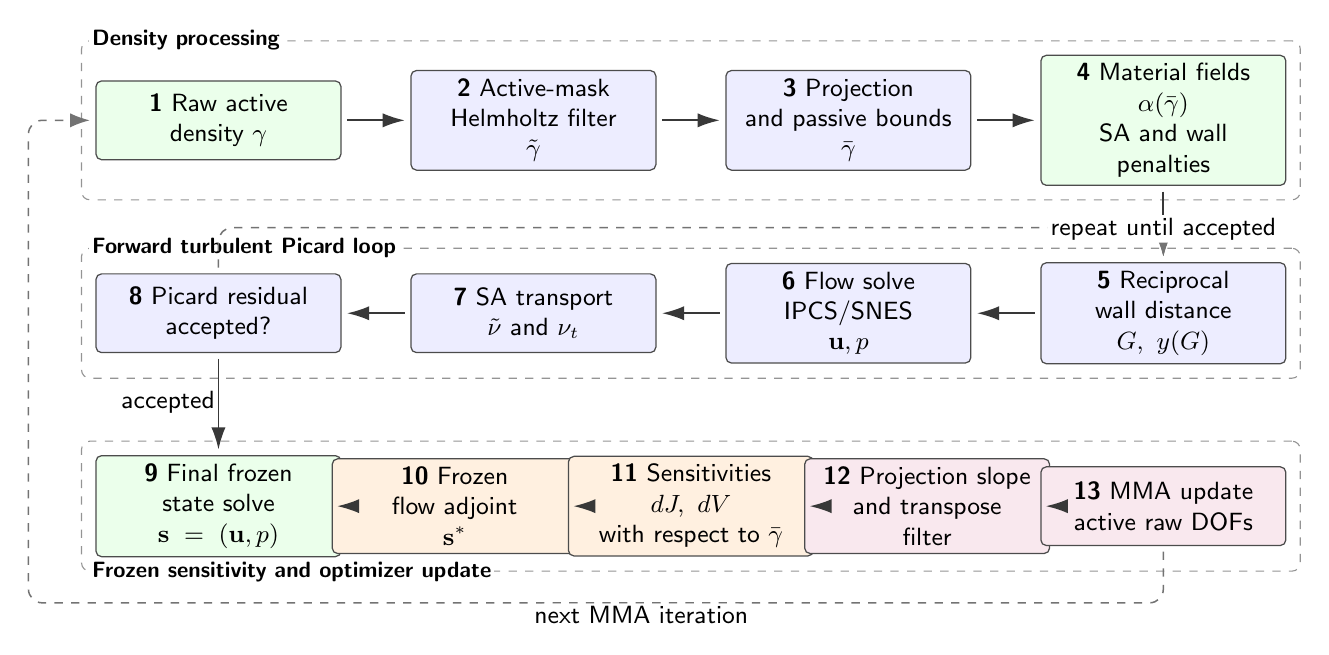
\begin{tikzpicture}[
  font=\sffamily\small,
  box/.style={
    draw=black!70,
    rounded corners=2pt,
    line width=0.45pt,
    align=center,
    minimum height=10mm,
    text width=29mm,
    inner sep=3pt,
    fill=white
  },
  process/.style={box, fill=blue!7},
  state/.style={box, fill=green!8},
  adjoint/.style={box, fill=orange!12},
  update/.style={box, fill=purple!9},
  arrow/.style={-{Latex[length=2.8mm,width=1.8mm]}, line width=0.62pt, draw=black!78, shorten <=2pt, shorten >=2pt},
  looparrow/.style={-{Latex[length=2.5mm,width=1.8mm]}, line width=0.55pt, draw=black!55, dashed, rounded corners=5pt, shorten <=2pt, shorten >=2pt},
  group/.style={draw=black!42, rounded corners=3pt, dashed, inner sep=5pt}
]

% Row 1: density processing, left to right.
\node[state]   (raw)        at (0.0,  0.0) {\textbf{1} Raw active\\density $\gamma$};
\node[process] (filter)     at (4.0,  0.0) {\textbf{2} Active-mask\\Helmholtz filter\\$\tilde{\gamma}$};
\node[process] (projection) at (8.0,  0.0) {\textbf{3} Projection\\and passive bounds\\$\bar{\gamma}$};
\node[state]   (physics)    at (12.0, 0.0) {\textbf{4} Material fields\\$\alpha(\bar{\gamma})$\\SA and wall penalties};

% Row 2: forward turbulent Picard loop, right to left.
\node[process] (wall)   at (12.0,-2.45) {\textbf{5} Reciprocal\\wall distance\\$G,\ y(G)$};
\node[process] (flow)   at (8.0, -2.45) {\textbf{6} Flow solve\\IPCS/SNES\\$\mathbf{u},p$};
\node[process] (sa)     at (4.0, -2.45) {\textbf{7} SA transport\\$\tilde{\nu}$ and $\nu_t$};
\node[process] (accept) at (0.0, -2.45) {\textbf{8} Picard residual\\accepted?};

% Row 3: frozen sensitivity and optimizer update, left to right.
\node[state]   (final)     at (0.0, -4.90) {\textbf{9} Final frozen\\state solve\\$\mathbf{s}=(\mathbf{u},p)$};
\node[adjoint] (adj)       at (3.0, -4.90) {\textbf{10} Frozen\\flow adjoint\\$\mathbf{s}^{*}$};
\node[adjoint] (sens)      at (6.0, -4.90) {\textbf{11} Sensitivities\\$dJ,\ dV$\\with respect to $\bar{\gamma}$};
\node[update]  (transpose) at (9.0, -4.90) {\textbf{12} Projection slope\\and transpose\\filter};
\node[update]  (mma)       at (12.0,-4.90) {\textbf{13} MMA update\\active raw DOFs};

\node[group, fit=(raw)(filter)(projection)(physics)] (g1) {};
\node[font=\sffamily\bfseries\footnotesize, fill=white, inner sep=1pt, anchor=west]
  at ($(g1.north west)+(0.1,0.0)$) {Density processing};

\node[group, fit=(wall)(flow)(sa)(accept)] (g2) {};
\node[font=\sffamily\bfseries\footnotesize, fill=white, inner sep=1pt, anchor=west]
  at ($(g2.north west)+(0.1,0.0)$) {Forward turbulent Picard loop};

\node[group, fit=(final)(adj)(sens)(transpose)(mma)] (g3) {};
\node[font=\sffamily\bfseries\footnotesize, fill=white, inner sep=1pt, anchor=west]
  at ($(g3.south west)+(0.1,0.0)$) {Frozen sensitivity and optimizer update};

\draw[arrow] (raw) -- (filter);
\draw[arrow] (filter) -- (projection);
\draw[arrow] (projection) -- (physics);
\draw[arrow] (physics.south) -- (wall.north);

\draw[arrow] (wall) -- (flow);
\draw[arrow] (flow) -- (sa);
\draw[arrow] (sa) -- (accept);
\draw[looparrow] (accept.north) -- ++(0,0.58) -|
  node[pos=0.73, above, fill=white, inner sep=1pt] {repeat until accepted}
  (wall.north);
\draw[arrow] (accept.south) -- node[pos=0.48, left, fill=white, inner sep=1pt] {accepted} (final.north);

\draw[arrow] (final) -- (adj);
\draw[arrow] (adj) -- (sens);
\draw[arrow] (sens) -- (transpose);
\draw[arrow] (transpose) -- (mma);
\draw[looparrow] (mma.south) -- ++(0,-0.72) -|
  node[pos=0.23, below, fill=white, inner sep=1pt] {next MMA iteration}
  ($(raw.west)+(-0.85,0)$) -- (raw.west);

\end{tikzpicture}
\end{document}
